\documentclass{article}
\usepackage[utf8]{inputenc}
\usepackage{amsmath}
\usepackage{graphicx}
\usepackage{wrapfig}
\usepackage{float}
\usepackage{dirtytalk}
\usepackage{setspace}
\usepackage{multirow}
\usepackage{array}
\usepackage[utf8]{inputenc}
\usepackage{amsmath}
\usepackage{graphicx}
\usepackage{wrapfig}
\usepackage{float}
\usepackage{dirtytalk}
\usepackage{setspace}
\usepackage{multirow}
\usepackage{array}
\usepackage[utf8]{inputenc}
\usepackage{natbib}
\usepackage{graphicx}
\usepackage{booktabs}
\usepackage{longtable}
\usepackage{array}
\usepackage{multirow}
\usepackage{wrapfig}
\usepackage{float}
\usepackage{colortbl}
\usepackage{pdflscape}
\usepackage{tabu}
\usepackage{threeparttable}
\usepackage{threeparttablex}
\usepackage[normalem]{ulem}
\usepackage{makecell}
\usepackage{xcolor}
\usepackage{gensymb}
\usepackage{amsmath}
\usepackage{amssymb}
\usepackage{tabularx}
\usepackage[colorinlistoftodos]{todonotes}
\usepackage[
backend=biber,
style=apa,
sorting=ynt
]{biblatex}
\usepackage{geometry}
\geometry{
 a4paper,
 total={150mm,237mm},
 left=30mm,
 top=30mm,
 }

 \usepackage{lineno}
 \usepackage[inline]{trackchanges}
 \linenumbers

\addbibresource{references2.bib}

\begin{document}



\section{Supporting information to: Pockmarks Enhance Submarine Groundwater Discharge and Seawater Intrusion with Magnitude Controlled by Geological Structure}

\subsection{Description of MODFLOW6 settings}
The MODFLOW6 groundwater flow and transport models were solved using the BICGSTAB solver with an HCLOSE and RCLOSE of 1$\times10^{-5}$ and a relaxation factor of 0.97.
Dispersion was modelled using the UPSTREAM weighting scheme. For all simulations, a constant time step was used. For the steady-state models, a time step of 1000 days was used.
For the sea-level rise scenarios, a timestep of 365 days was used. For the aquifer depletion scenarios, a time step of 1 day was used.

\subsection{Influence of vertical discretization on vertical salinity profiles}

To quantify the effect of numerical error/diffusion on the salinity profile in the aquitards, a simple numerical experiment was conducted. 
This was done by modeling the salinity distribution in a 1D vertical column of cells under various conditions using MODFLOW6.
The top cell represented the seafloor, to which a constant head and constant concentration condition was applied. 
The bottom cell represented the base of the Petone Marine Distal aquitard, to which a constant vertical flux of freshwater was applied and a constant concentration of 0 PSU. 
Models were run until a steady state was reached (Main text, Table 2), and with a constant density.
This configuration was run for low and high values of hydraulic conductivities, thickness, and fluxes, to represent the range of conditions at the locations where sediment core observations were taken. 
For the flux, the values chosen were $1\times10^{-5}$ m/day, approximately the rate of discharge within the pockmarks, and $2\times10^{-4}$ m/day, an extreme value representing a high point discharge or horizontal discharge into the pockmarks, given the anisotropy of the Petone Marine Distal (Main text, Table 1).
For the thickness, a minimum value of $5$ m and a maximum value of $15$ m were chosen (Main text, Figure 3b)
For each combination of these values, models were run with a vertical cell size of 0.5 m (the same as the vertical discretization of the full 3D model) and 0.01 m.
Comparing the salinity profiles for these two cell sizes reveals only a minimal difference, even in the uppermost cell of the aquitard at a depth of 0.25 m (Supporting Figure 1). This suggests that numerical error is not affecting the modeled values of salinity at the sediment core observation points.

\begin{figure}[h!]
\centering
\makebox[\textwidth][c]{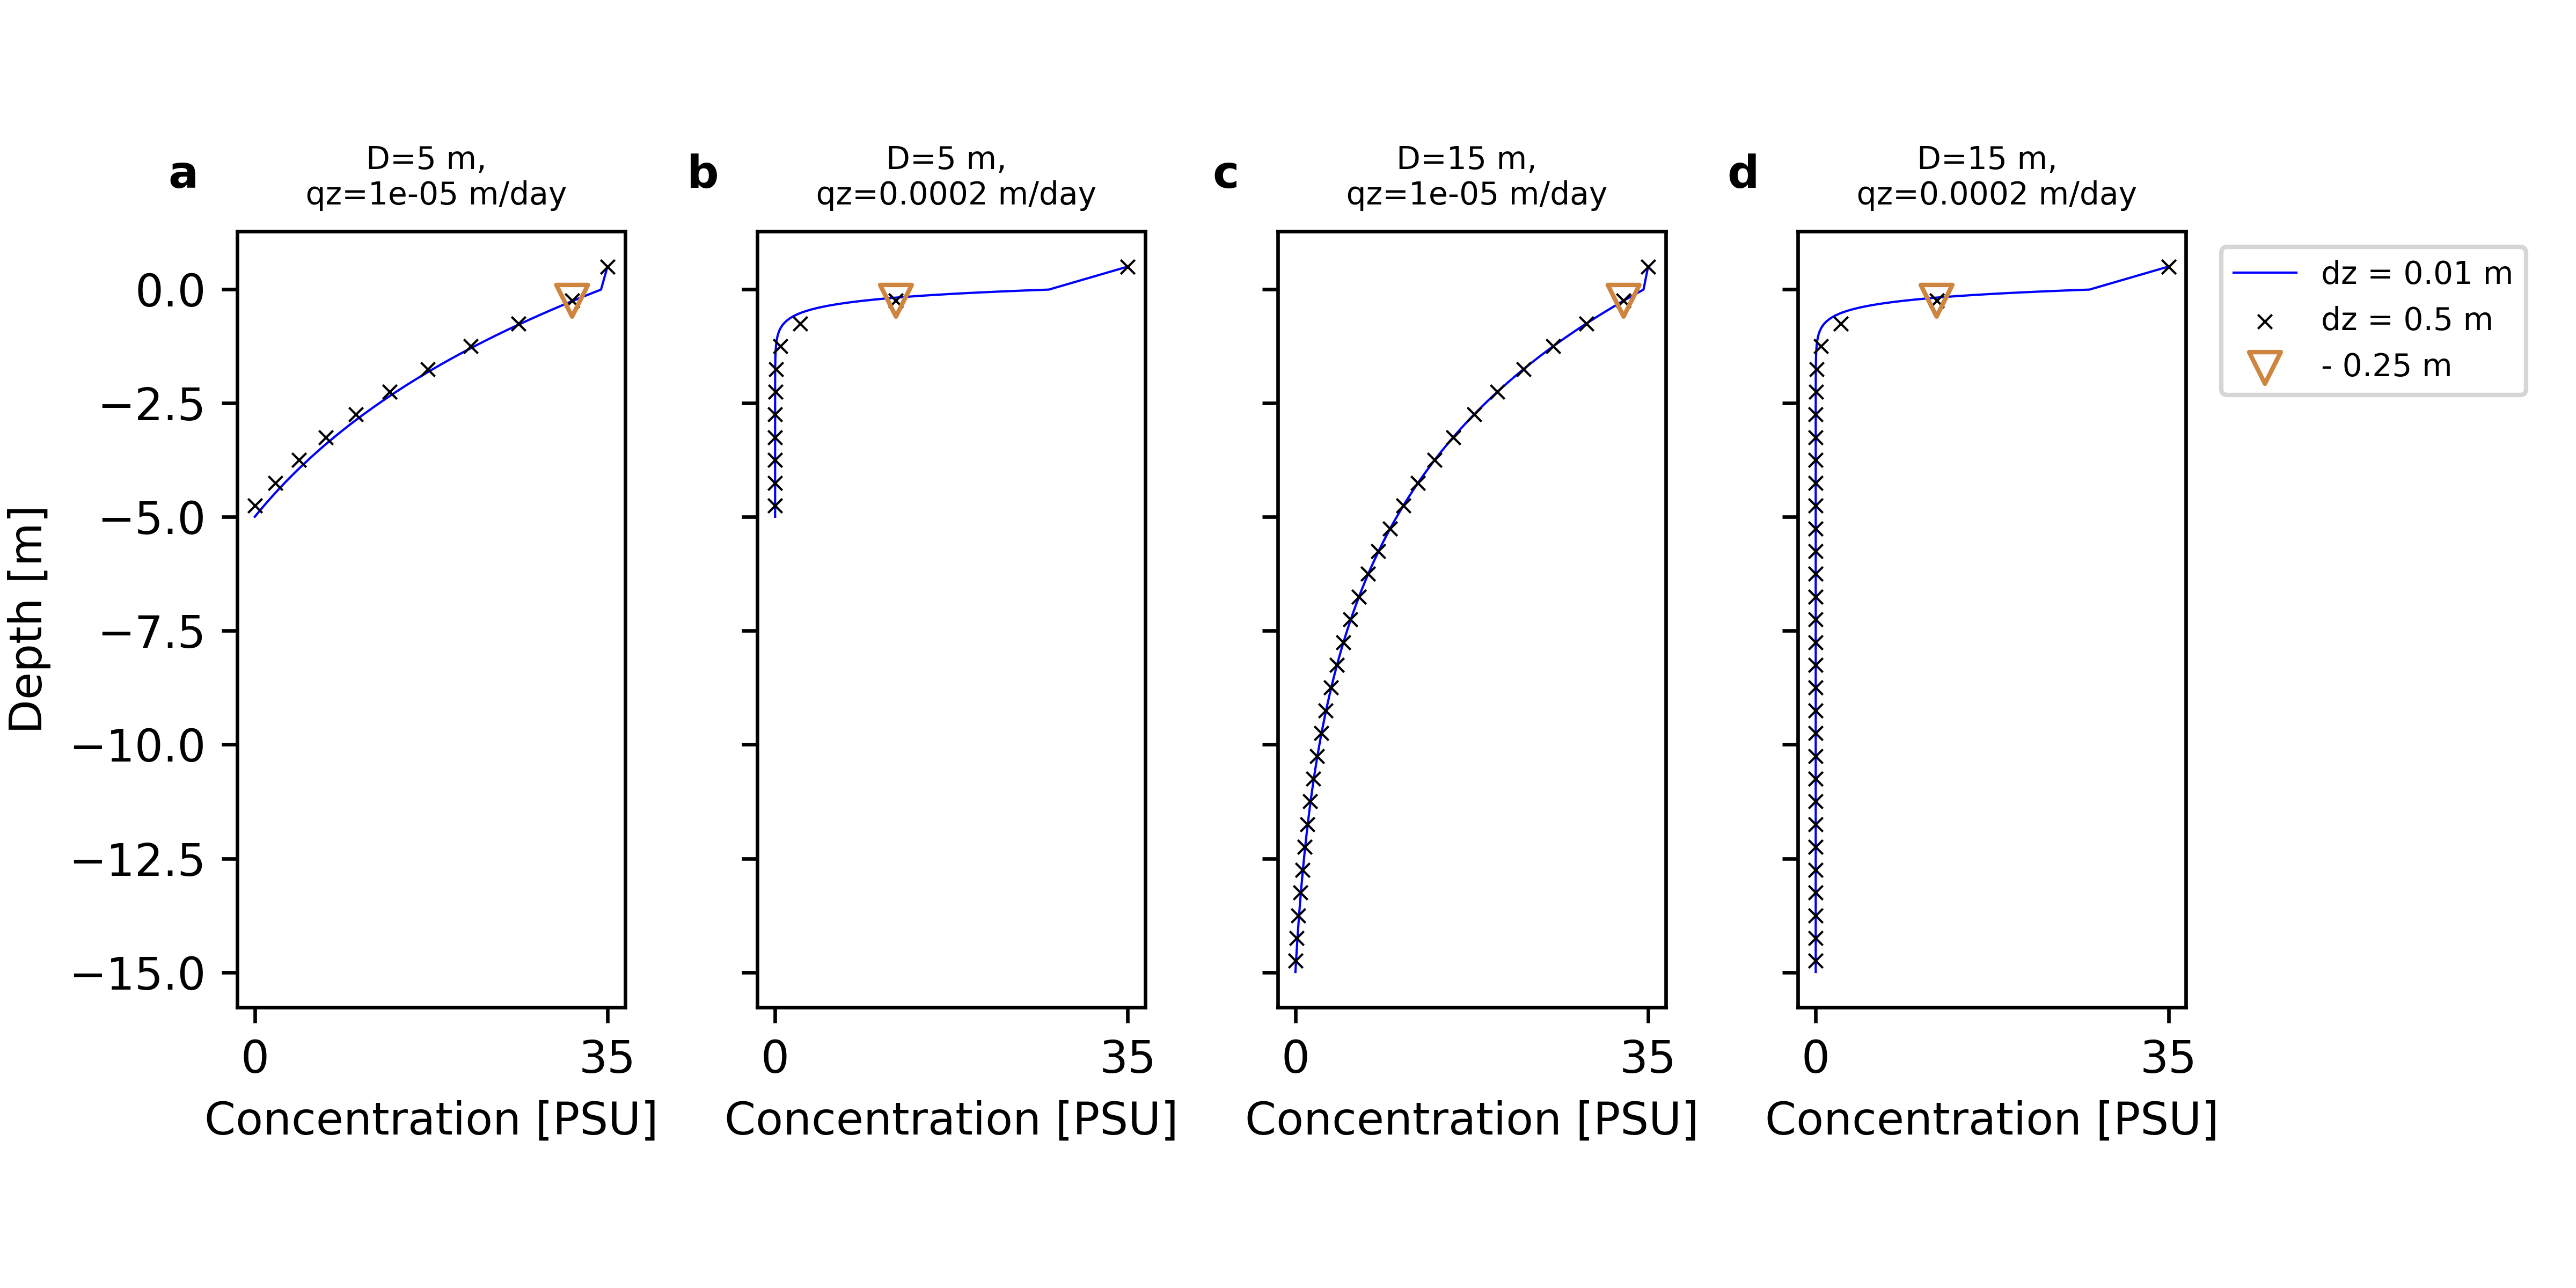
\includegraphics[width=1.2\textwidth]{1d_scenario_results.png}}
\caption{Comparison between concentration profiles in a 1D aquitard model for $dz=0.01$ m and $dz=0.5$ m.}
\label{fig:grid_sensitivity}
\end{figure}

\pagebreak

\subsection{Discharge in and around pockmarks for the Present-day scenario and Thin Aquitard model.}
To understand the influence of the bathymetry and thinning of the aquitard at the pockmarks, the salinity and rate of submarine discharge within the pockmarks (the areas defined in Figure 6a, main text) and in a 50 m buffer outside of these areas were compared (Supporting Table 1). For all pockmarks, submarine groundwater was discharged at a greater rate and with a lower salinity when compared to the area around them. 
\begin{table}[h]
\centering
\caption{Rate and salinity of submarine groundwater discharge inside the six pockmarks, compared to in a 50 m buffer around them for the Thin Aquitard model. In this conceptual model, the hydraulic conductivity of the aquitard is assumed to be uniform.}
\begin{tabular}{lllllll}
\hline
Pockmark \# & 1 & 2 & 3 & 4 & 5 & 6 \\
\hline 
Specific discharge inside [$\times10^{-5}$ m/day]  & 0.69 & 1.0 & 0.75 & 0.82 & 1.1& 1.6\\
Specific discharge outside [$\times10^{-5}$ m/day] & 0.28& 0.41 & 0.45 & 0.44 & 0.54 & 0.63\\
Average salinity within [PSU] & 28.6 & 26.6 & 28.1 & 27.7 & 25.2 & 22.5 \\
Average salinity outside [PSU] & 29.4 & 29.7 & 29.4 & 29.4 & 28.7 & 28.1 \\
\hline
\end{tabular}
\label{tab:table_stages}
\end{table}

\pagebreak
\subsection{Present-day scenario with Patchy Aquitard and Aquitard Conduits models}

\begin{figure}[h!]
\centering
\makebox[\textwidth][c]{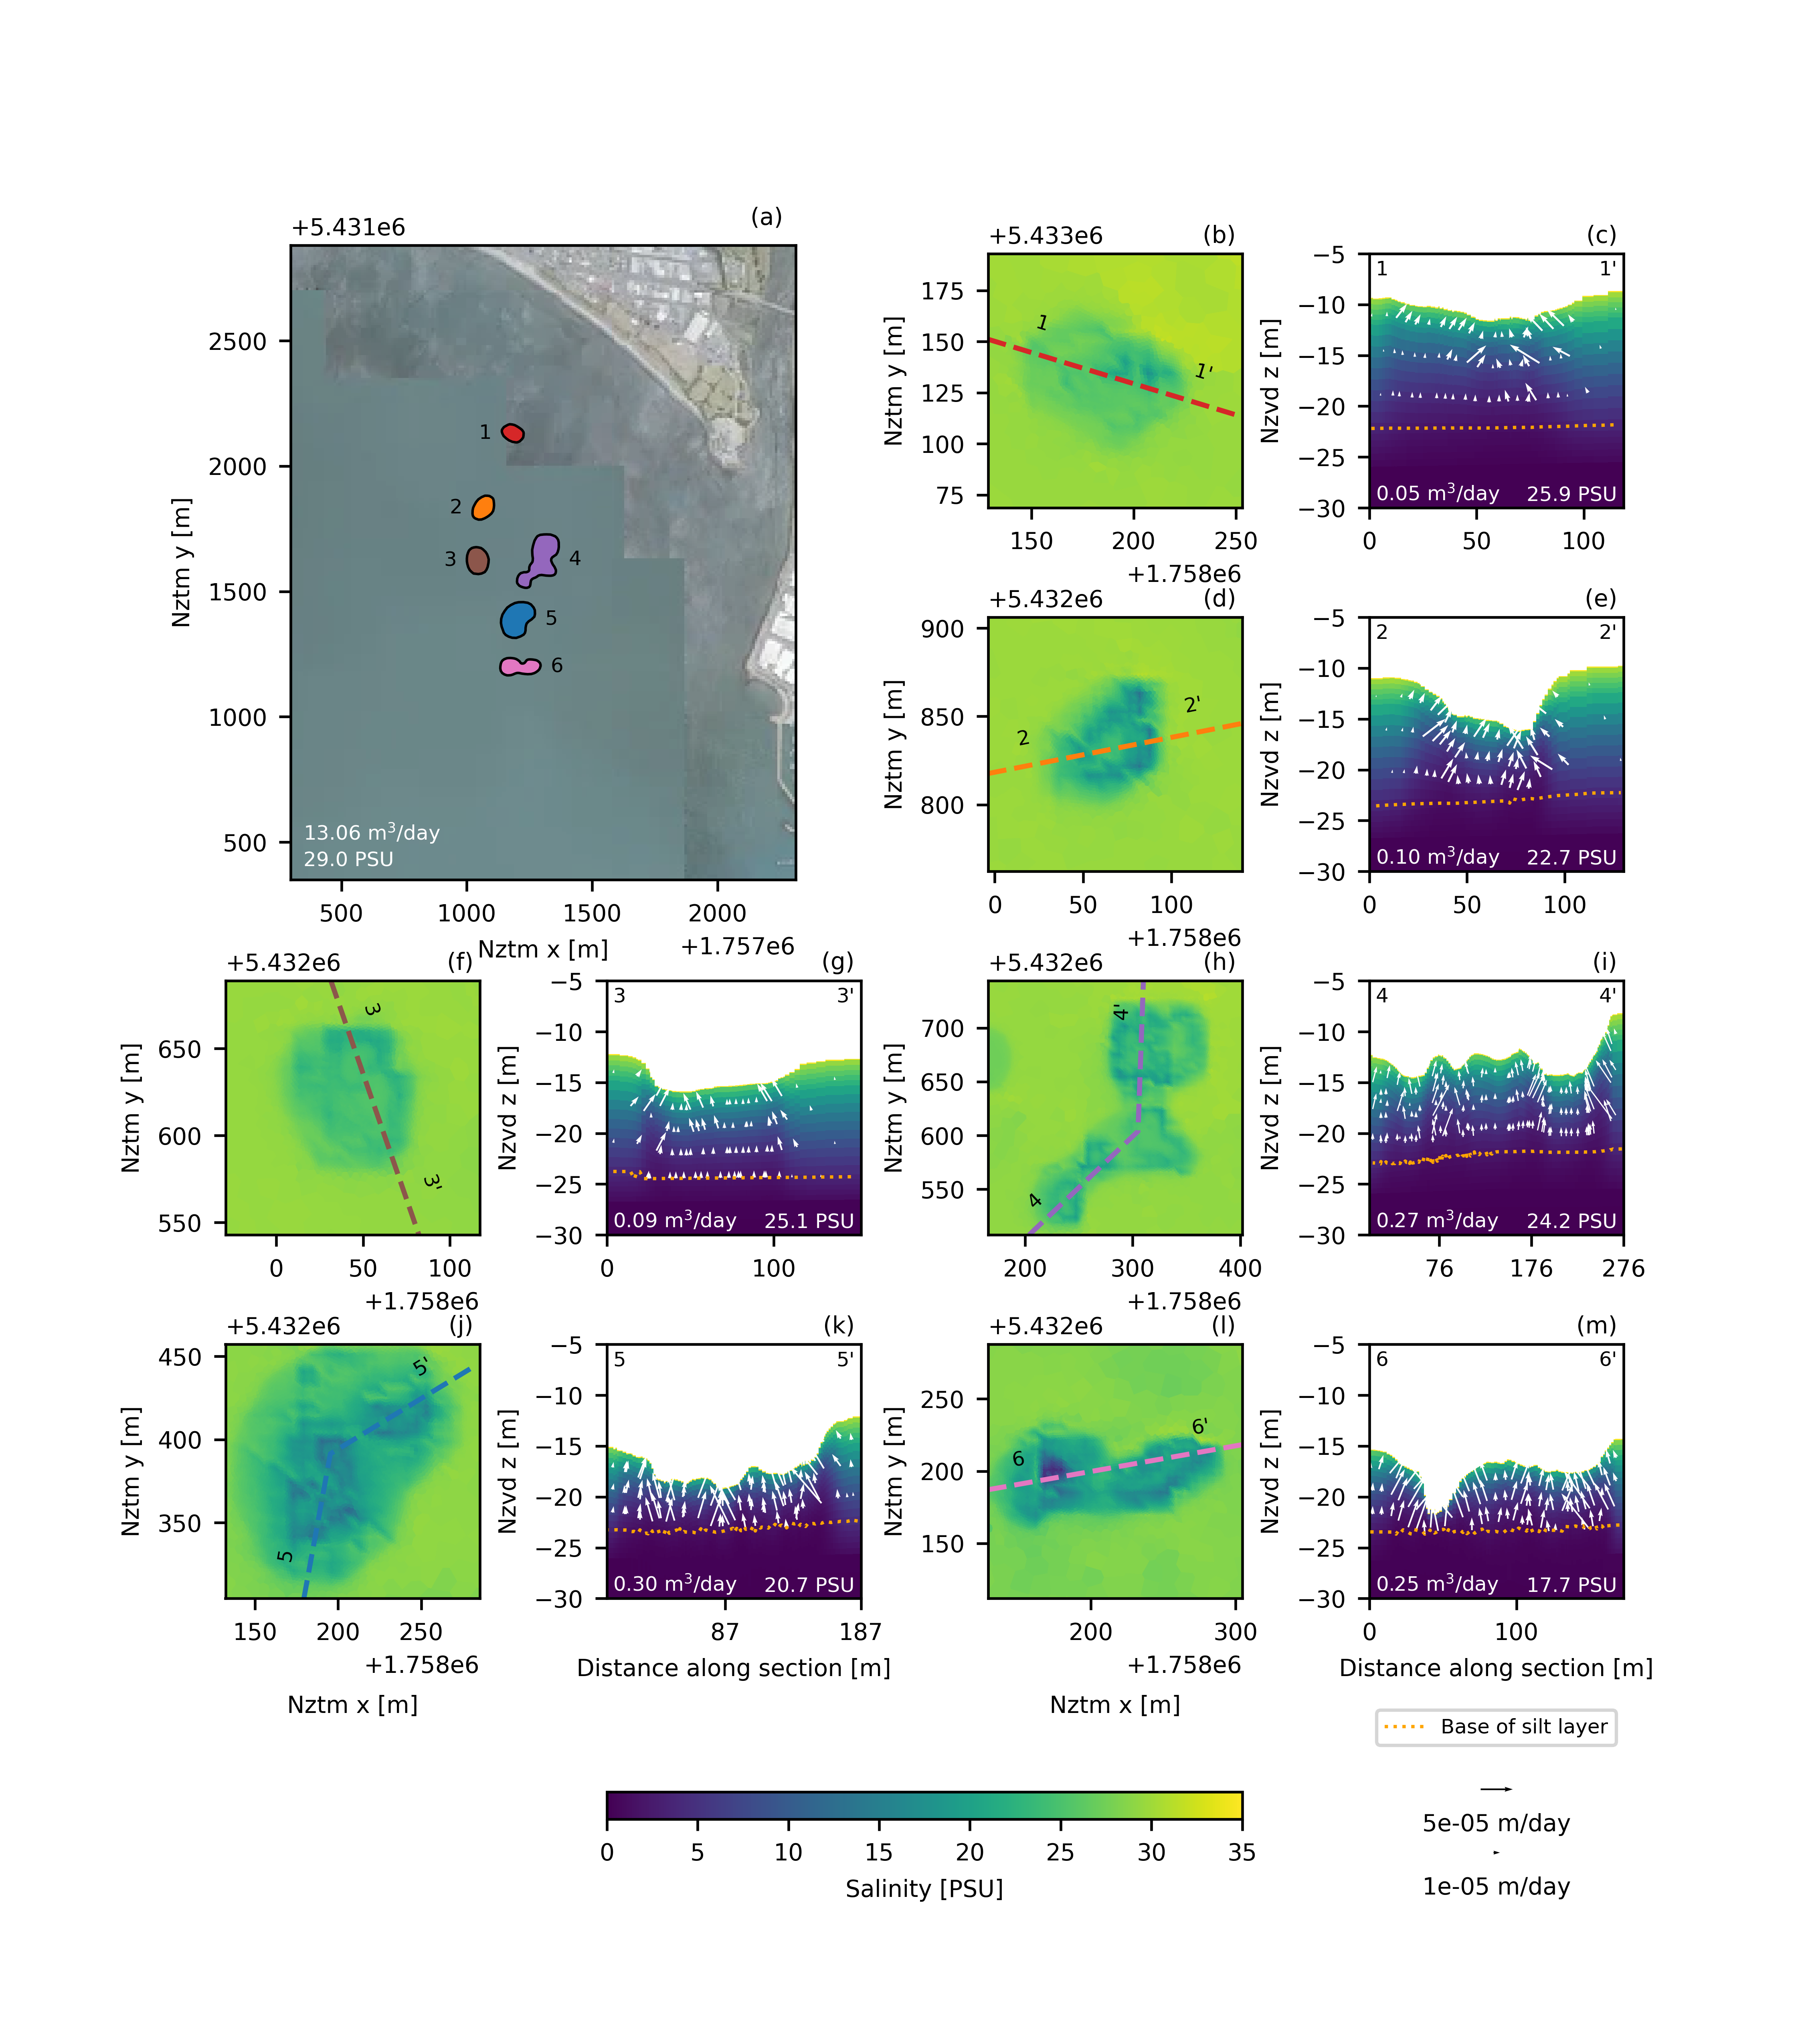
\includegraphics[width=1.1\textwidth]{hk1ave_r1_pockmark_salinity.png}}
\caption{Modeled salinity distributions and discharge at six pockmarks for the present-day using the Patchy Aquitard model.}
\label{fig_pockmarks_present_day}
\end{figure}

\begin{figure}[h!]
\centering
\makebox[\textwidth][c]{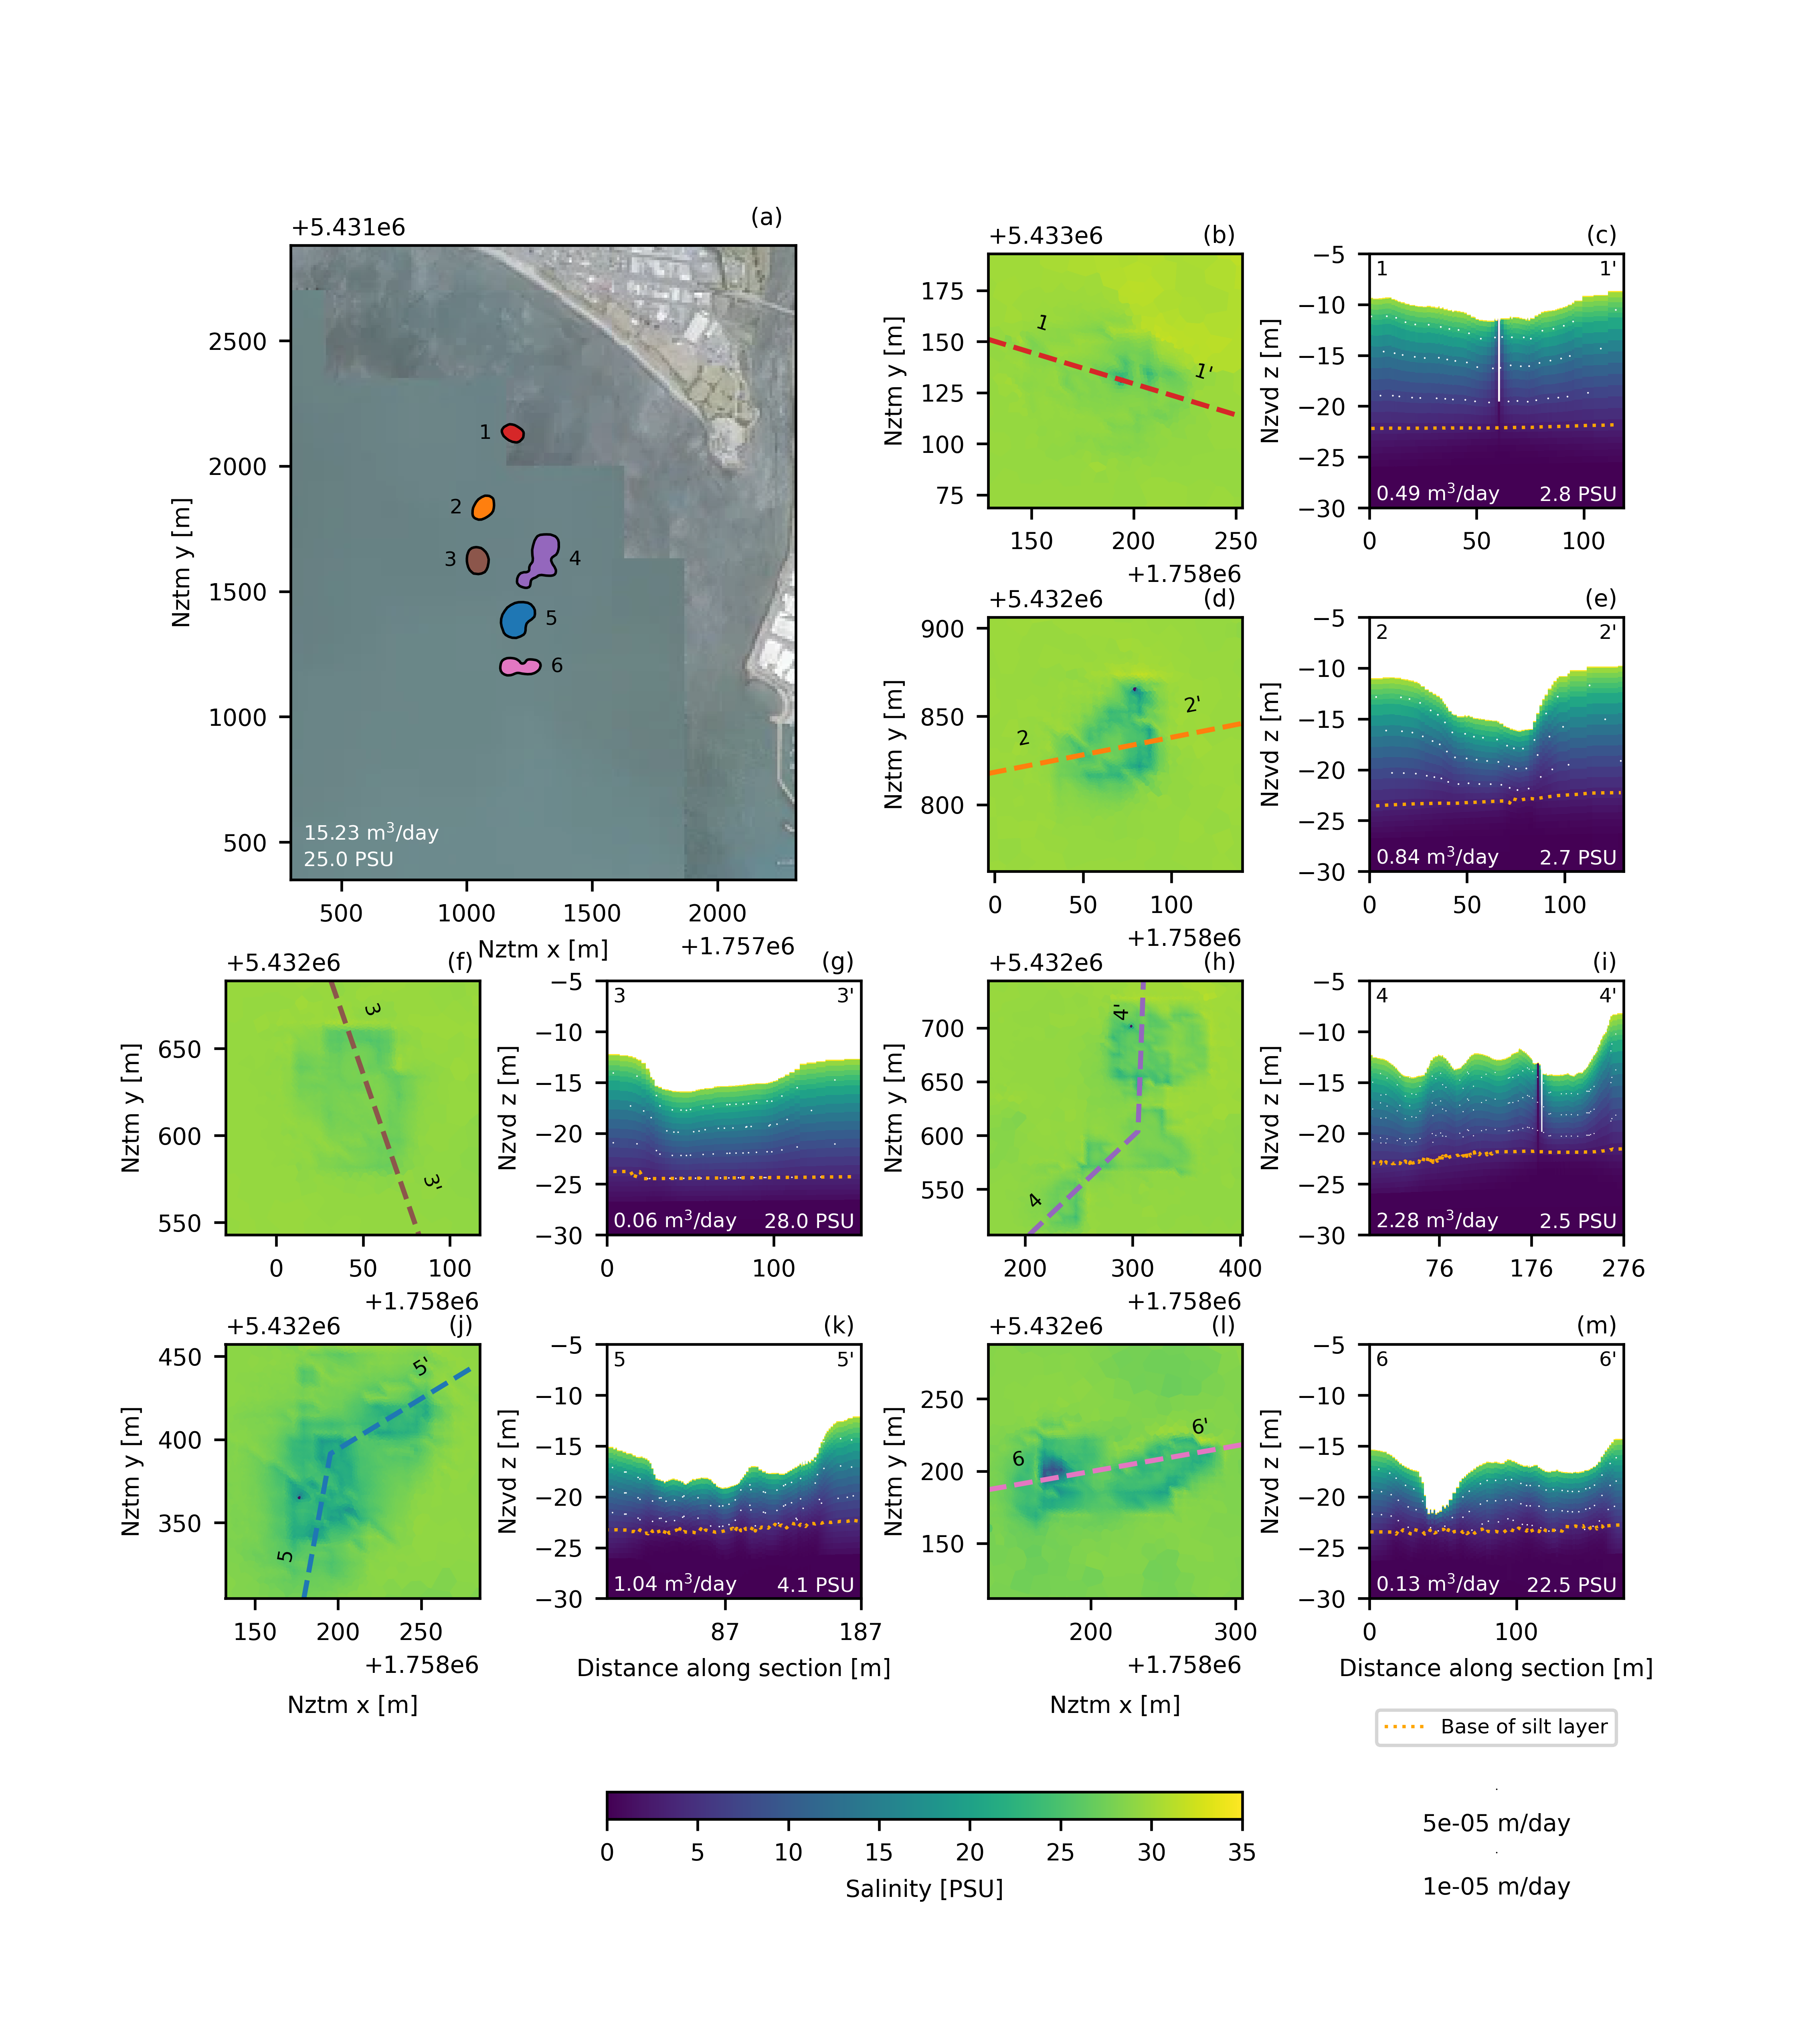
\includegraphics[width=1.1\textwidth]{c1ave_r1_pockmark_salinity.png}}
\caption{Modeled salinity distributions and discharge at six pockmarks for the present-day using the Aquitard Conduits model.}
\label{fig_pockmarks_present_day}
\end{figure}

\pagebreak
\subsection{Short-term model runs at steady-state with tidal forcing}
To investigate the influence of tidal forcing on the salinity and flux at measurement points, two additional scenarios were run.
The first was for the Thin Aquitard model, and the second was for the Aquitard Conduits model.
Both models used the conditions at the end of their respective steady-state models (Scenario 1 in the Main Text).
The effects of this tidal forcing on the flux and salinity at measurement points in the top layer of the Petone Marine aquitard is analysed.
Note that while in the main text a Conduit $K$ of 1 m/day was used, for this tidal forcing scenario a Conduit $K$ of 10 m/day was used.
It would be expected that the higher hydraulic conductivity of the conduits would lead to a greater tidal response, and therefore a more pronounced effect on the salinity and flux at the measurement points.

\noident Models were run for 10 tidal cycles (\~5 days). Each tidal cycle was discretized into 12 stress periods. Heads were calculated using a sinusoidal function.
The head at the seafloor boundary was varied around the mean level of -0.14 m with an amplitude of 0.8 m, reflecting a tidal range of 1.6 m (\cite{gyopari_lower_2014}). For the onshore and offshore aquitard boundaries, the head was prescribed based on the previously reported tidal response of the Upper Waiwhetu aquifer at the McEwan Park and Somes Island monitoring wells (Main Text Figure 2). For the offshore boundary, this had an amplitude of 0.7 m and no time lag. For the onshore boundary, this had an amplitude of 0.56 m and a time lag of 30 minutes. \\

\noindent For the Thin Aquitard model, no variation in the salinity at MC2-1, MC2-2, and MC2-3 was observed (Figure \ref{fig:tidal_thin}a).  However, for the flux at SV1 and SV2, the effects of tidal pumping can be seen, with fluxes reversing through the tidal cycle (Figure \ref{fig:tidal_thin}b). This is likely due to the low hydraulic diffusivity of the aquitard. For the Aquitard Conduits model, small variations in the salinity at the measurement points can be observed (Figure \ref{fig:tidal_conduits}a). Likewise, flux at the measurement points varies with the tidal cycle (Figure \ref{fig:tidal_conduits}b). However, unlike the Thin Aquitard model, this does not lead to a flow reversal (due to the higher hydraulic diffusivity of the conduits). Rather, the tidal forcing leads to lower and higher rates of discharge through the cycle, which is consistent with the observations of \cite{harding_characteristics_2000}. 

\begin{figure}[h!]
\centering
\makebox[\textwidth][c]{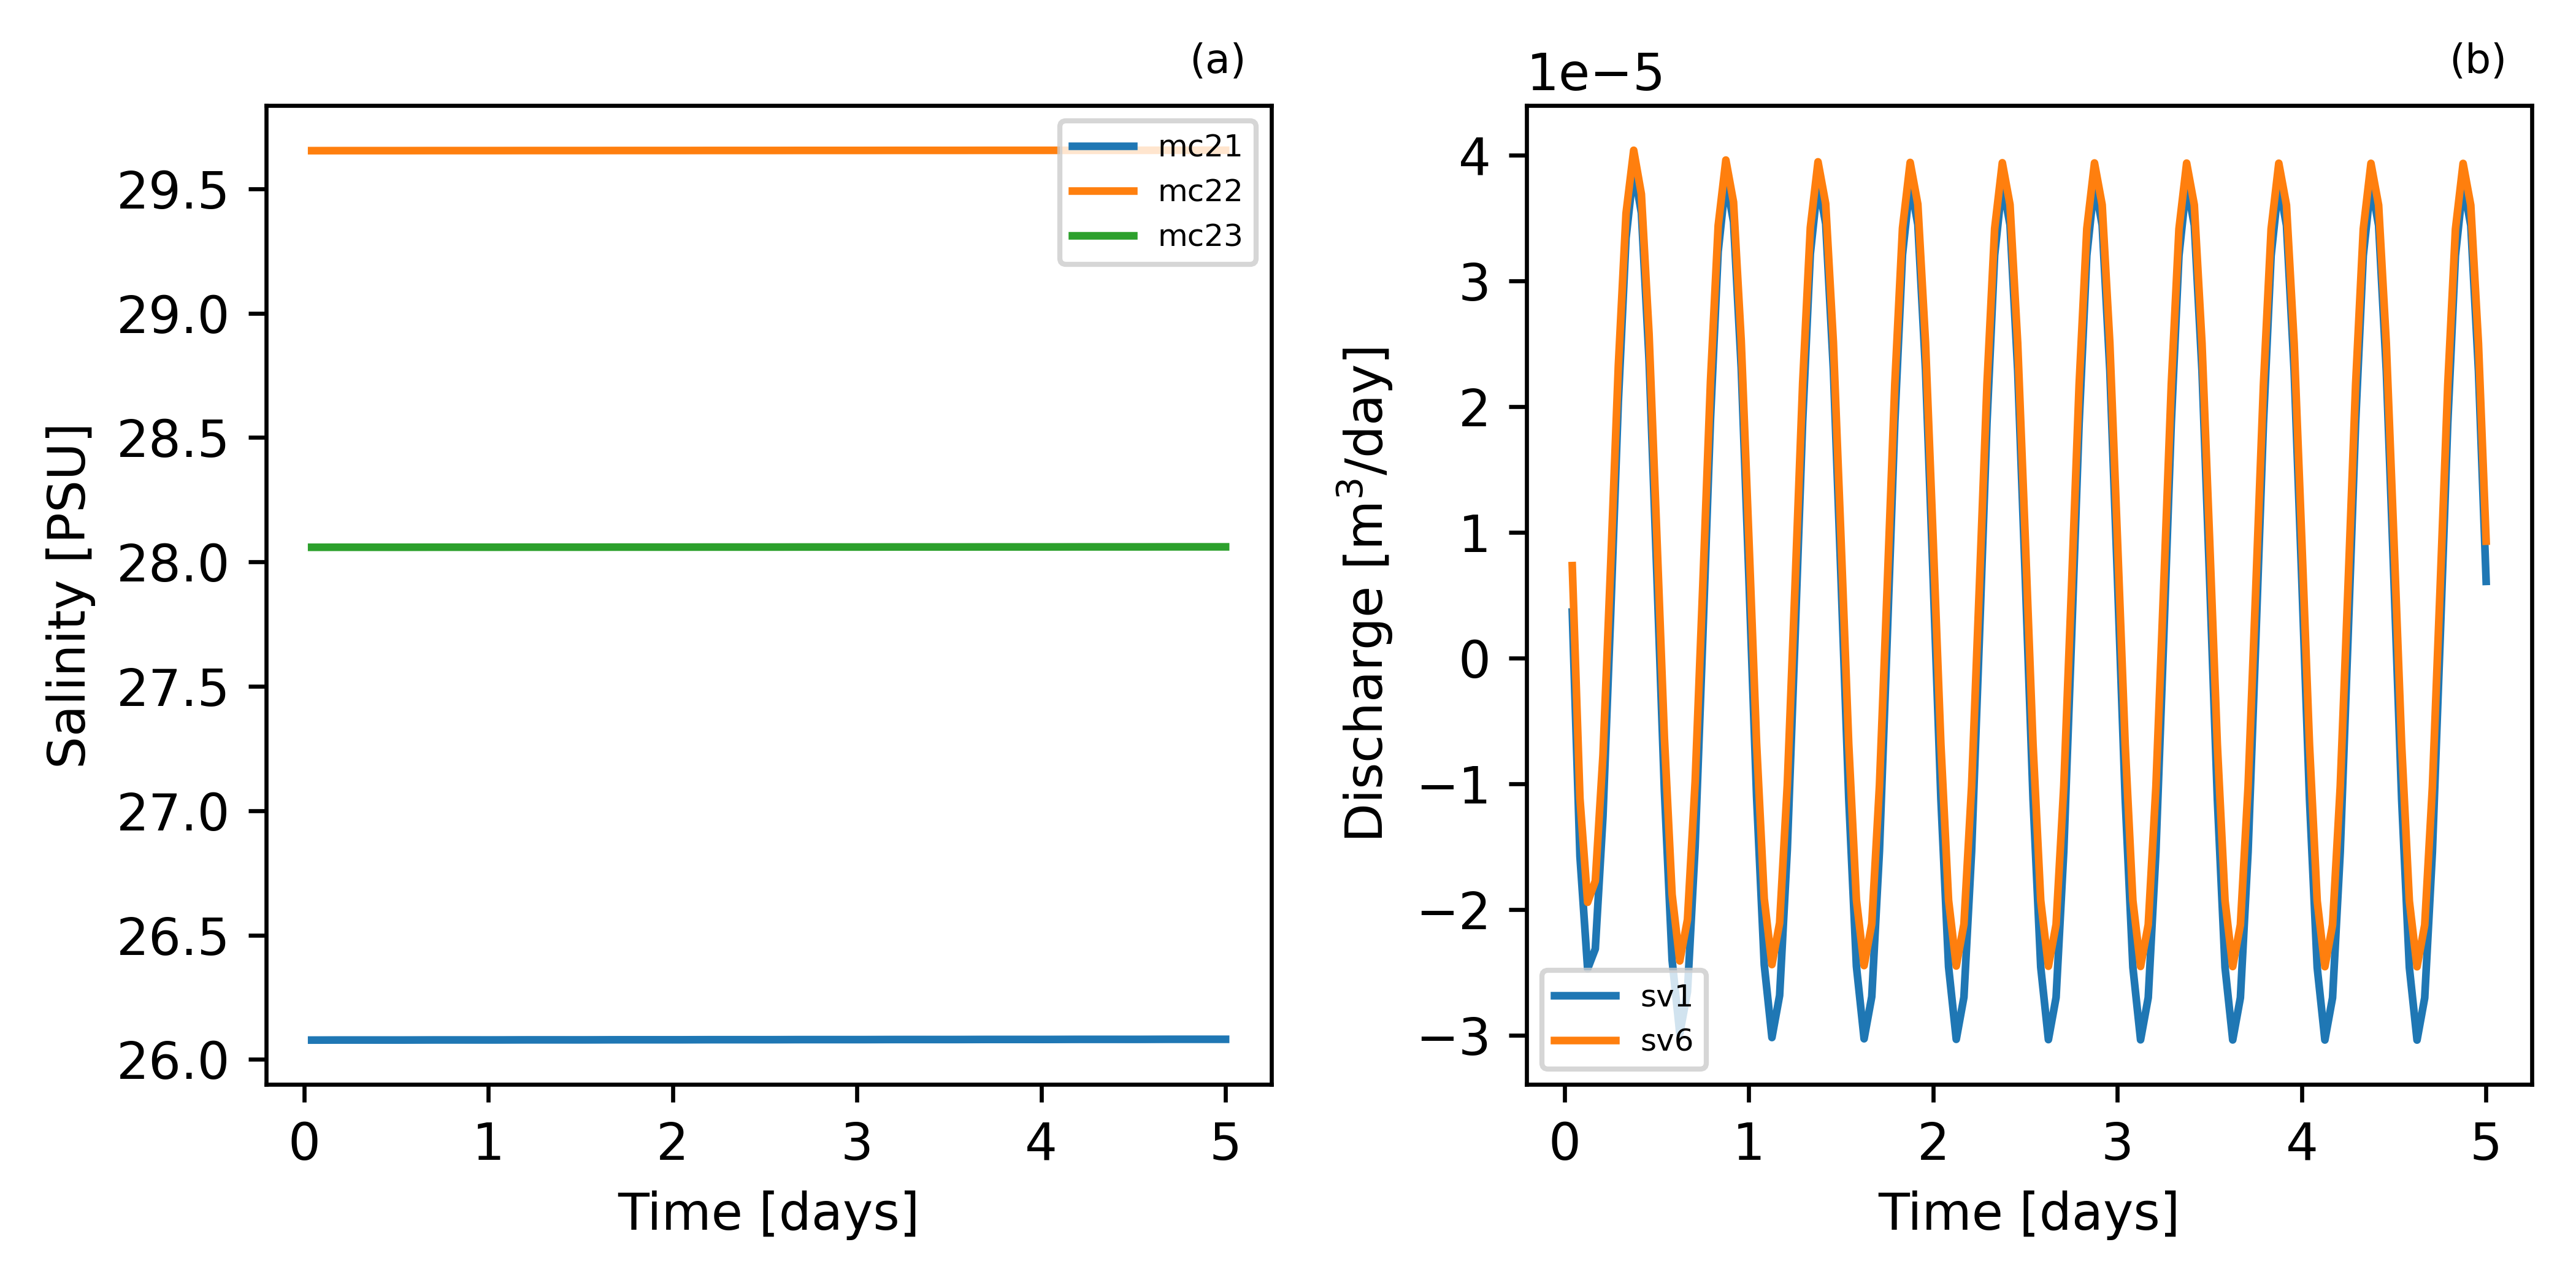
\includegraphics[width=0.7\textwidth]{tidal_effects_on_salinity_and_discharge_tidal_all_b.png}}
\caption{Modelled response of the (a) salinity and (b) flux to tidal oscillation at the measurement points for the Thin Aquitard Model}
\label{fig:tidal_thin}
\end{figure}

\begin{figure}[h!]
\centering
\makebox[\textwidth][c]{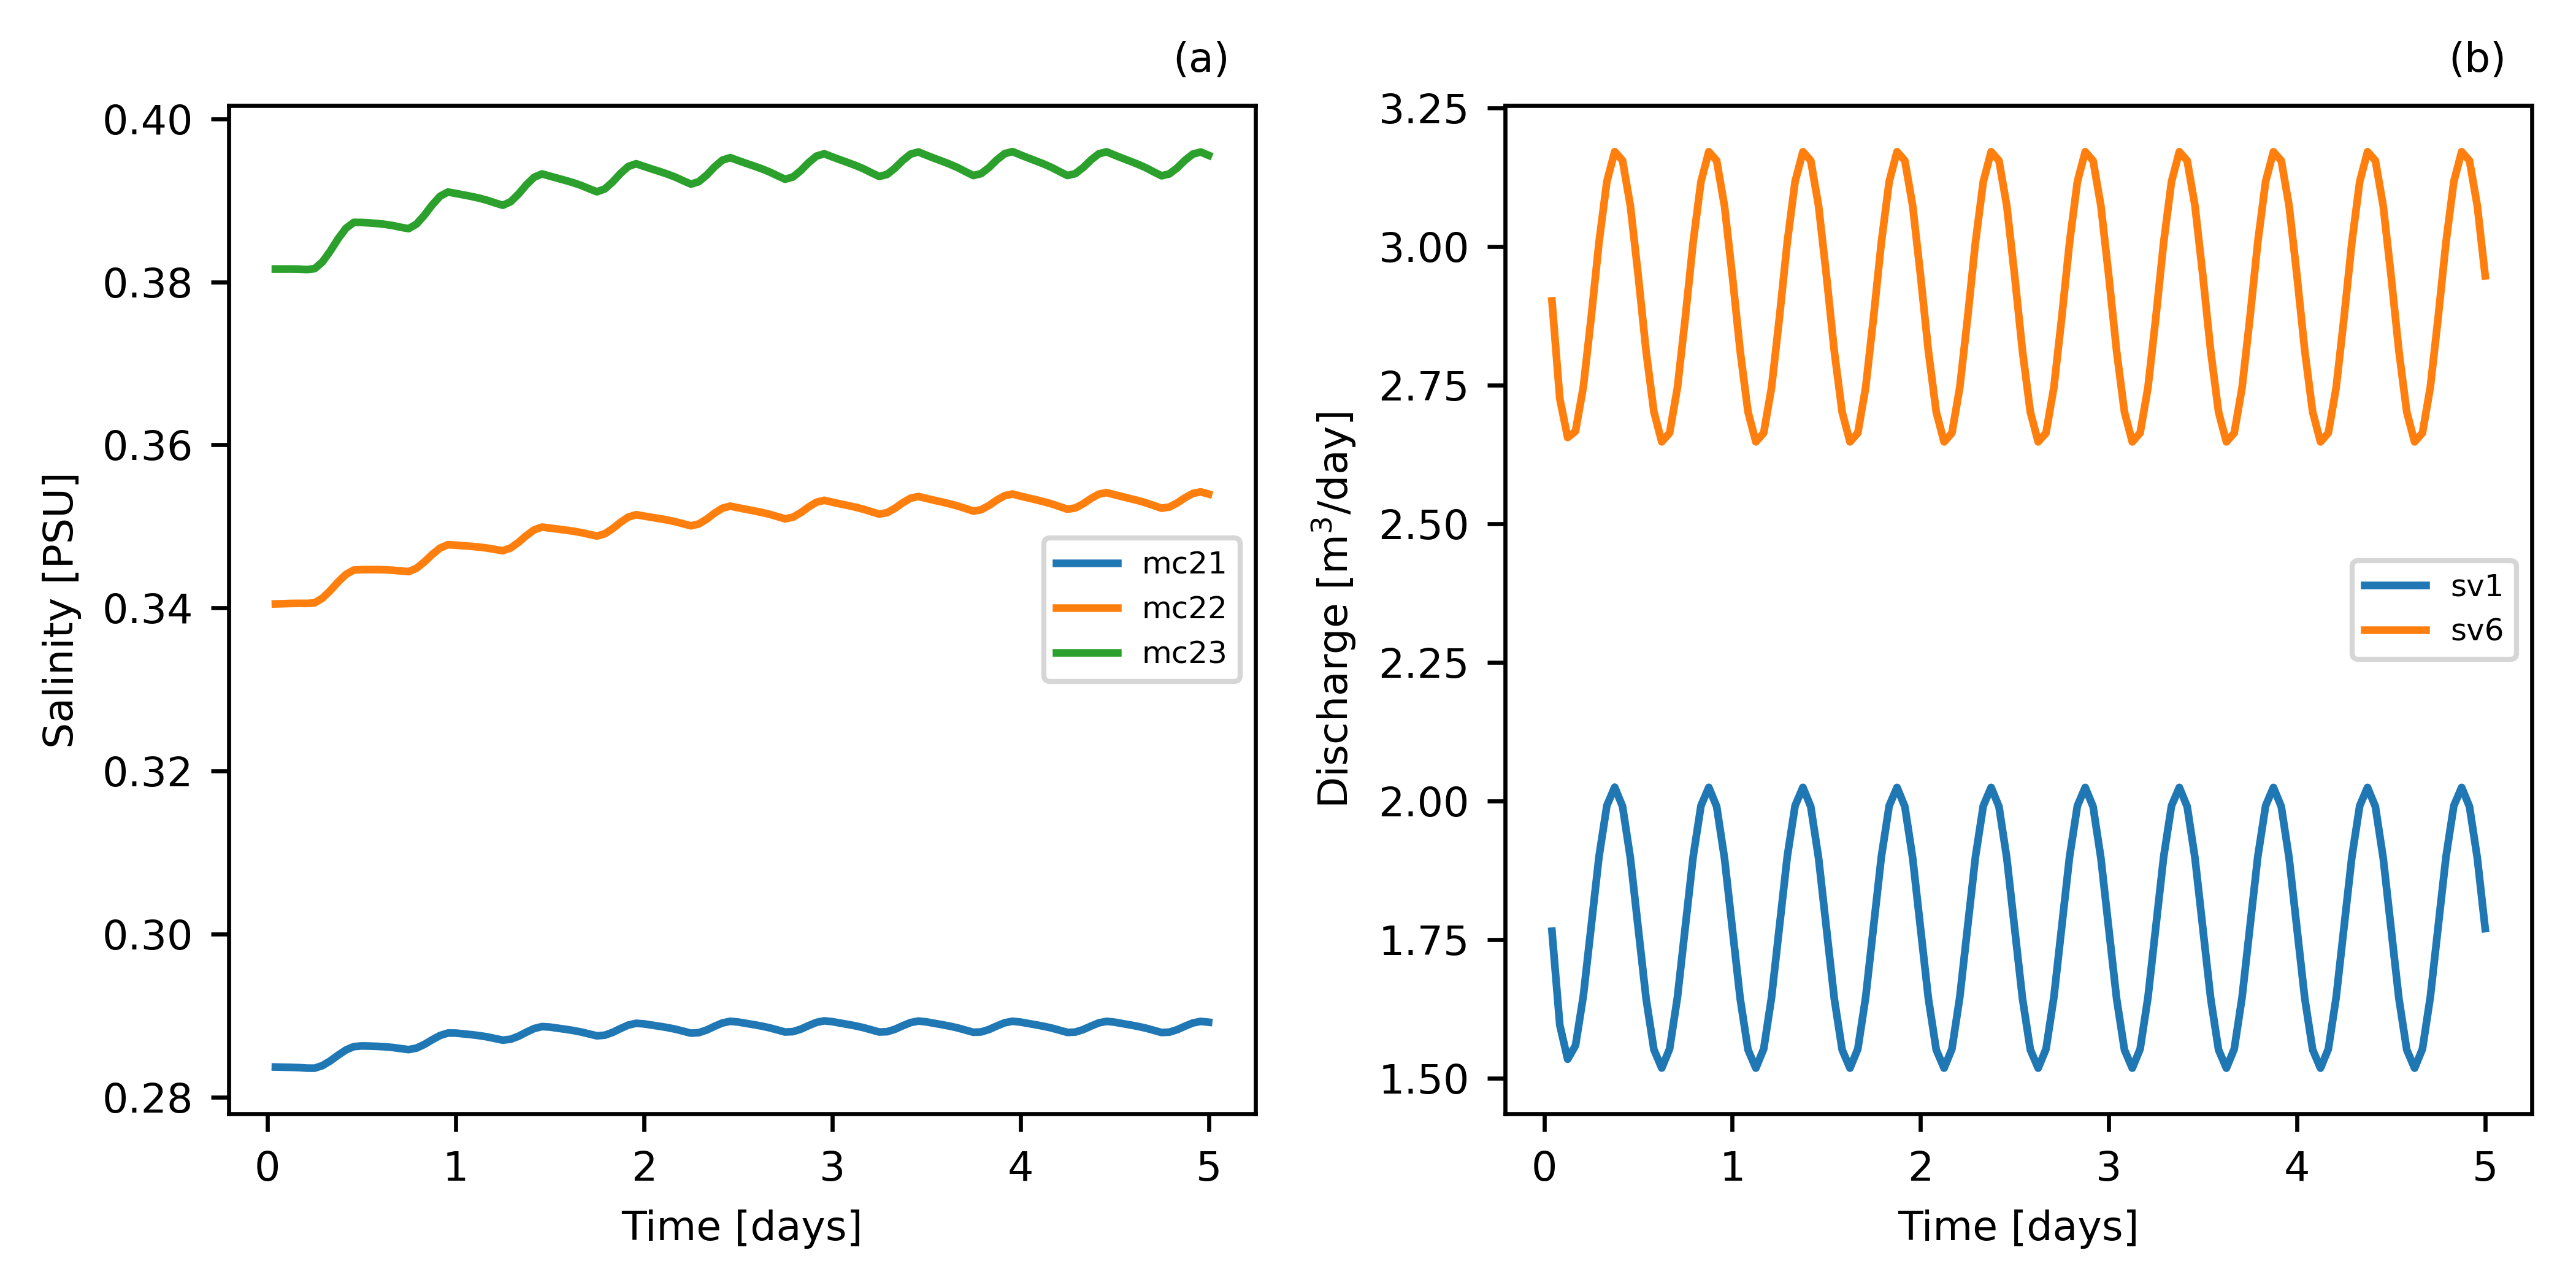
\includegraphics[width=0.7\textwidth]{tidal_effects_on_salinity_and_discharge_tidal_all_c.png}}
\caption{Modelled response of the (a) salinity and (b) flux to tidal oscillation at the measurement points for the Aquitard Conduits Model}
\label{fig:tidal_conduits}
\end{figure}

\subsection{Steady-state Scenario for the Thin Aquitard Model Including the effects of dispersion}

\noindent To explore the effects of dispersion on the salinity and flux at the observation points, three additional models were run.
These were the steady-state scenarios for each of the three conceptual models of pockmark structure.
The longitudinal dispersion ($\alpha_L$) was set to 10 m, the transverse dispersion ($\alpha_T$) was set to 1 m, and the vertical dispersion ($\alpha_V$) was set to 0.1 m (\cite{zech_is_2015}).
All other parameters were kept the same as the original model, where $\alpha_L, \alpha_T, \alpha_V = 0$ m.
Note that while in the main text a Conduit $K$ of 1 m/day was used, for this tidal forcing scenario a Conduit $K$ of 10 m/day was used.
The effect of dispersion for a lower hydraulic conductivity of the conduits is expected to be similar, possibly with an even larger effect on salinity, due to the relatively lower effect of advection.


\begin{figure}[h!]
\centering
\makebox[\textwidth][c]{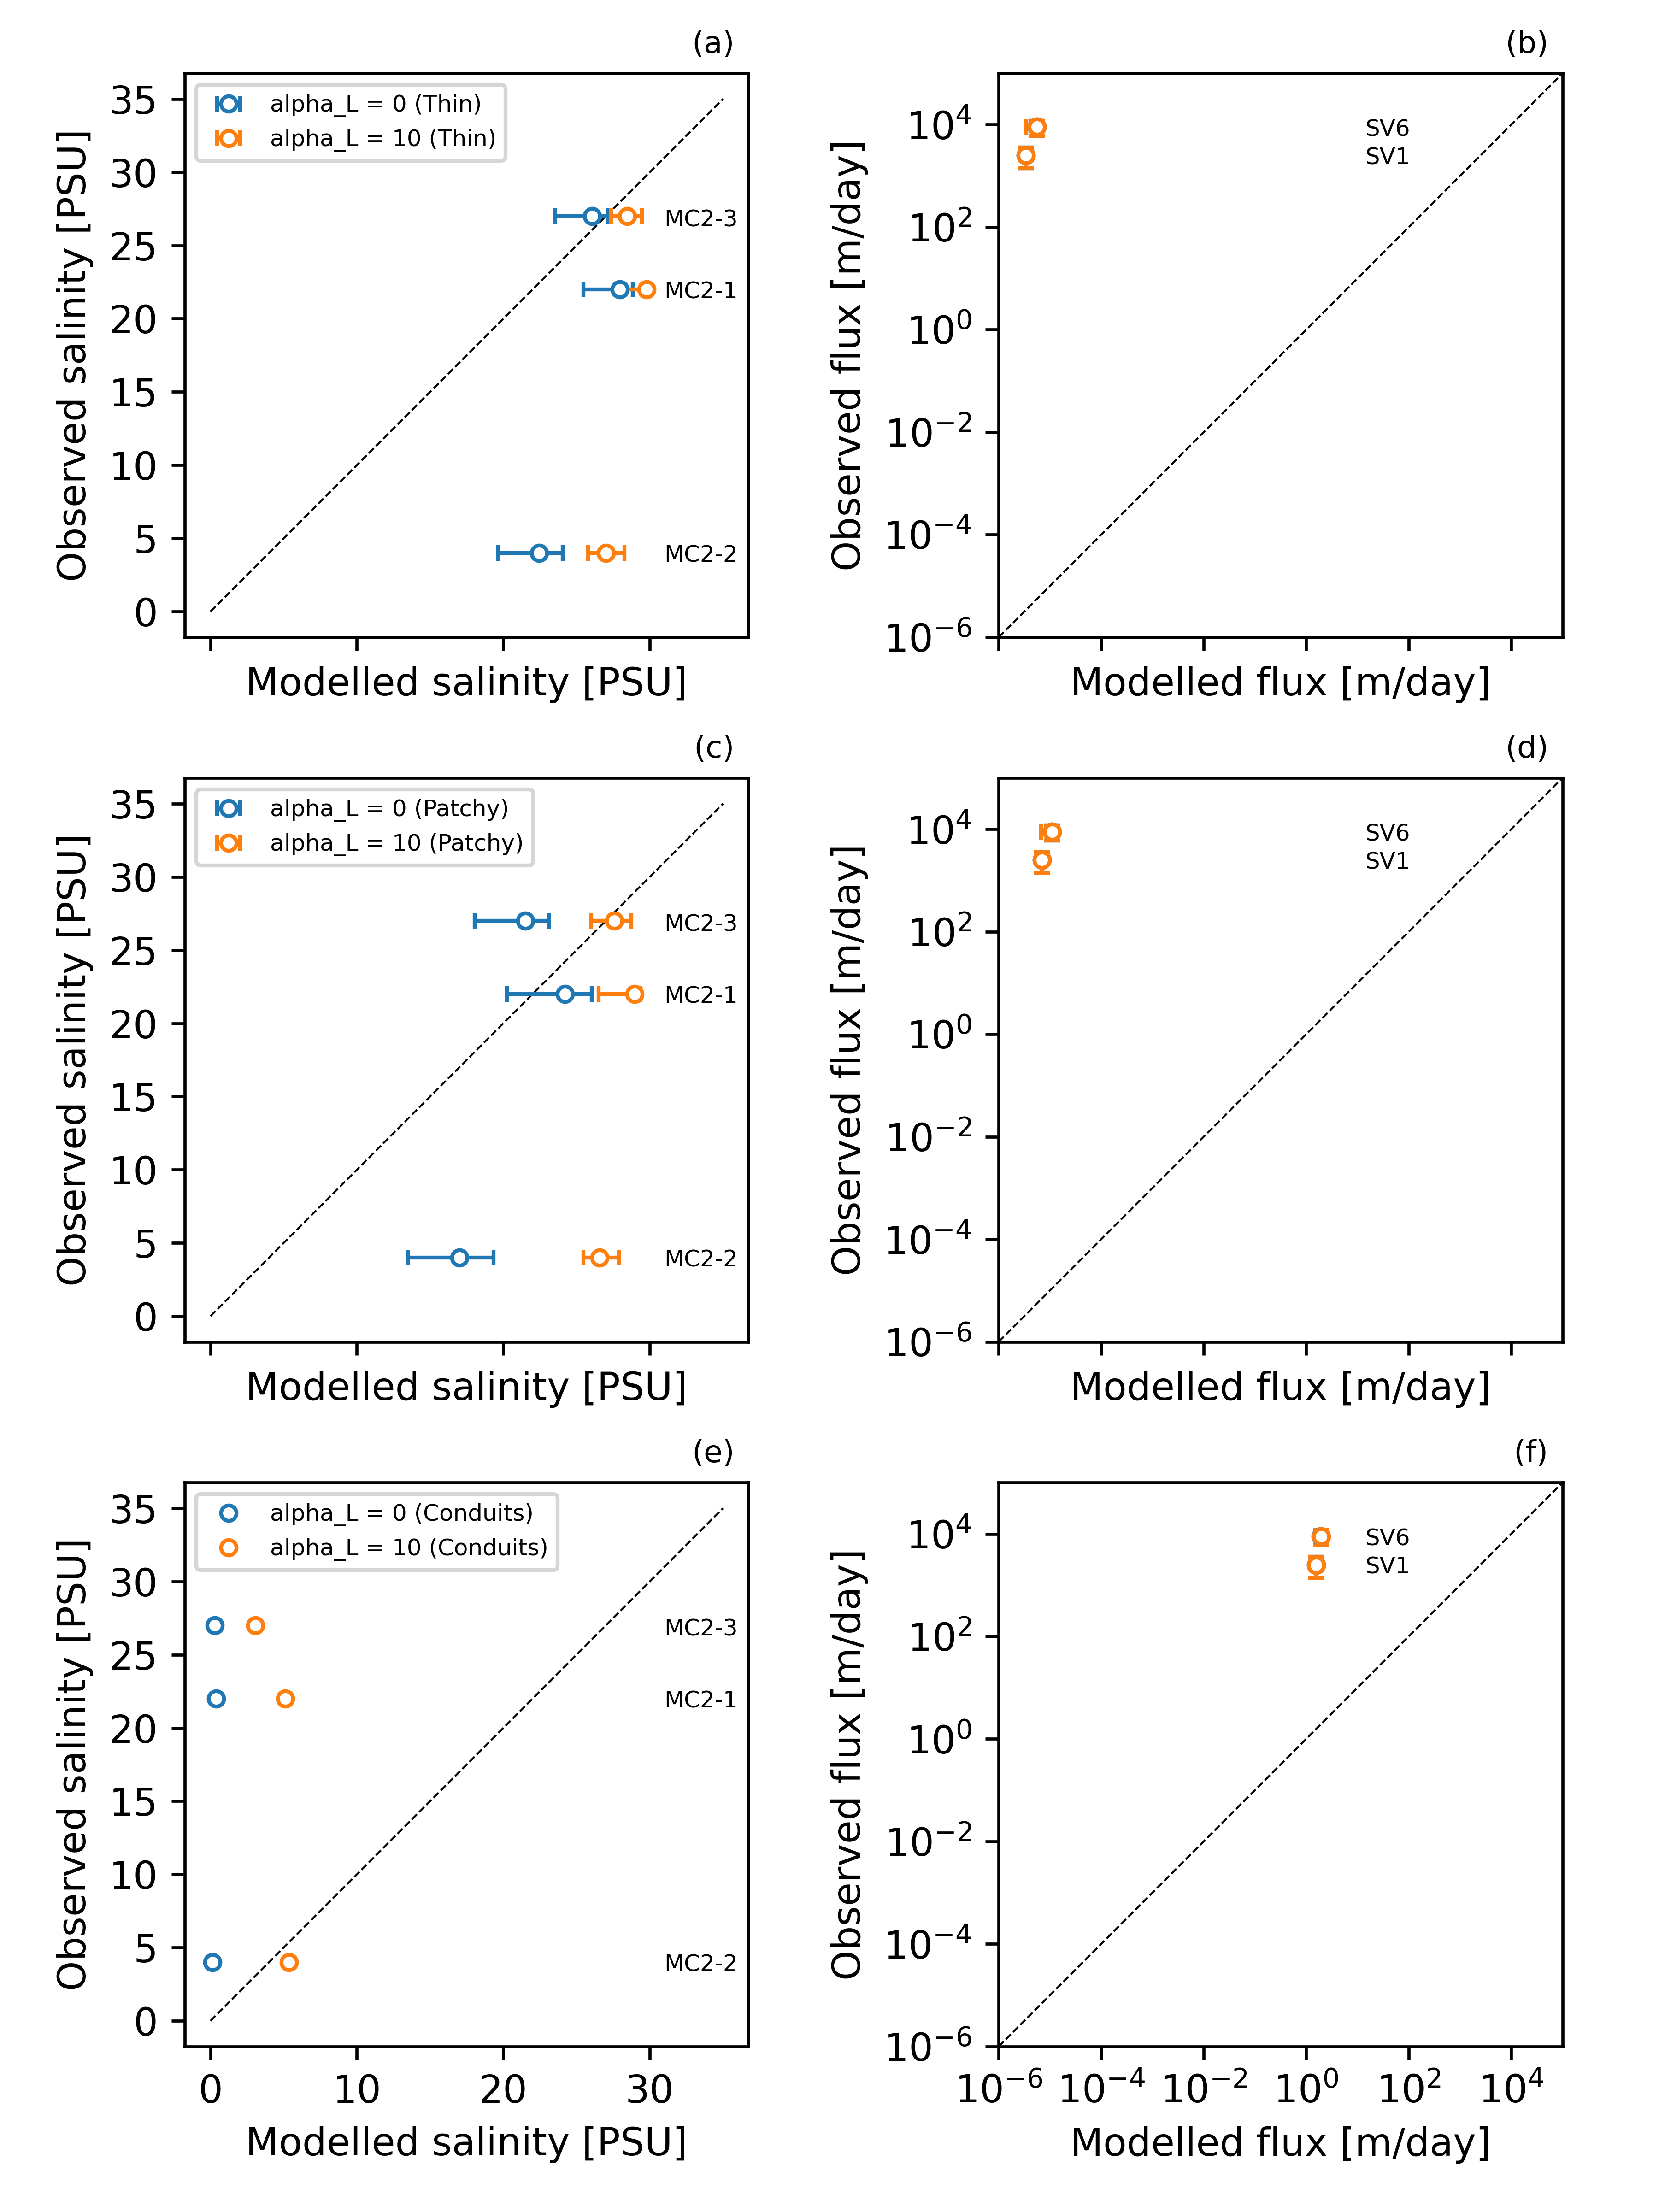
\includegraphics[width=0.8\textwidth]{compare_salinity_at_measurement_points_dispersion.png}}
\caption{Steady-state scenario with and without dispersion for the three conceptual models of pockmark structure. Note that for subplots b, d, and f, the blue markers appear behind the orange markers.}
\label{fig:tidal_conduits}
\end{figure}

\\

\noindent For the models with dispersion, salinity at the observation points was higher than for the models without dispersion (Figure 6a,c,e).
This difference was greatest for observation MC2-2, and was generally larger for the Patchy Aquitard (around 5 PSU to 10 PSU, see Figure 6b) and Aquitard Conduits (around 3 PSU to 6 PSU, see Figure 6f) models than for the Thin Aquitard Model (around 2 PSU to 5 PSU, see Figure 6a). For all three conceptual models, dispersion had no effect on the modelled flux at the observation points (Figure 6b,d,f).\\

\noindent Given the known effects of upstream dispersion (\cite{ irvine_upstream_2021}), this increase in salinity could be caused by back dispersion from the boundary condition, or lateral dispersion from areas around the measurement point with higher salinity.

\subsection{Additional scenarios}
To understand the influence of the hydraulic conductivity of the pockmarks in the Patchy Aquitard model,
an extra model was run where the vertical hydraulic conductivity in the patches was increased by a factor of 100 to $1.8 \times 10^{-3}$ m/day.
Again, a higher Conduit $K$ of 10 m/day was used for this scenario, which is expected to increase the amount of seawater intrusion into the aquitard.
For the Present-day scenario, this additional model showed good agreement with the low salinity observed at MC2-2 (Supporting Figure 4).
\\

\begin{figure}[h!]
\centering
\makebox[\textwidth][c]{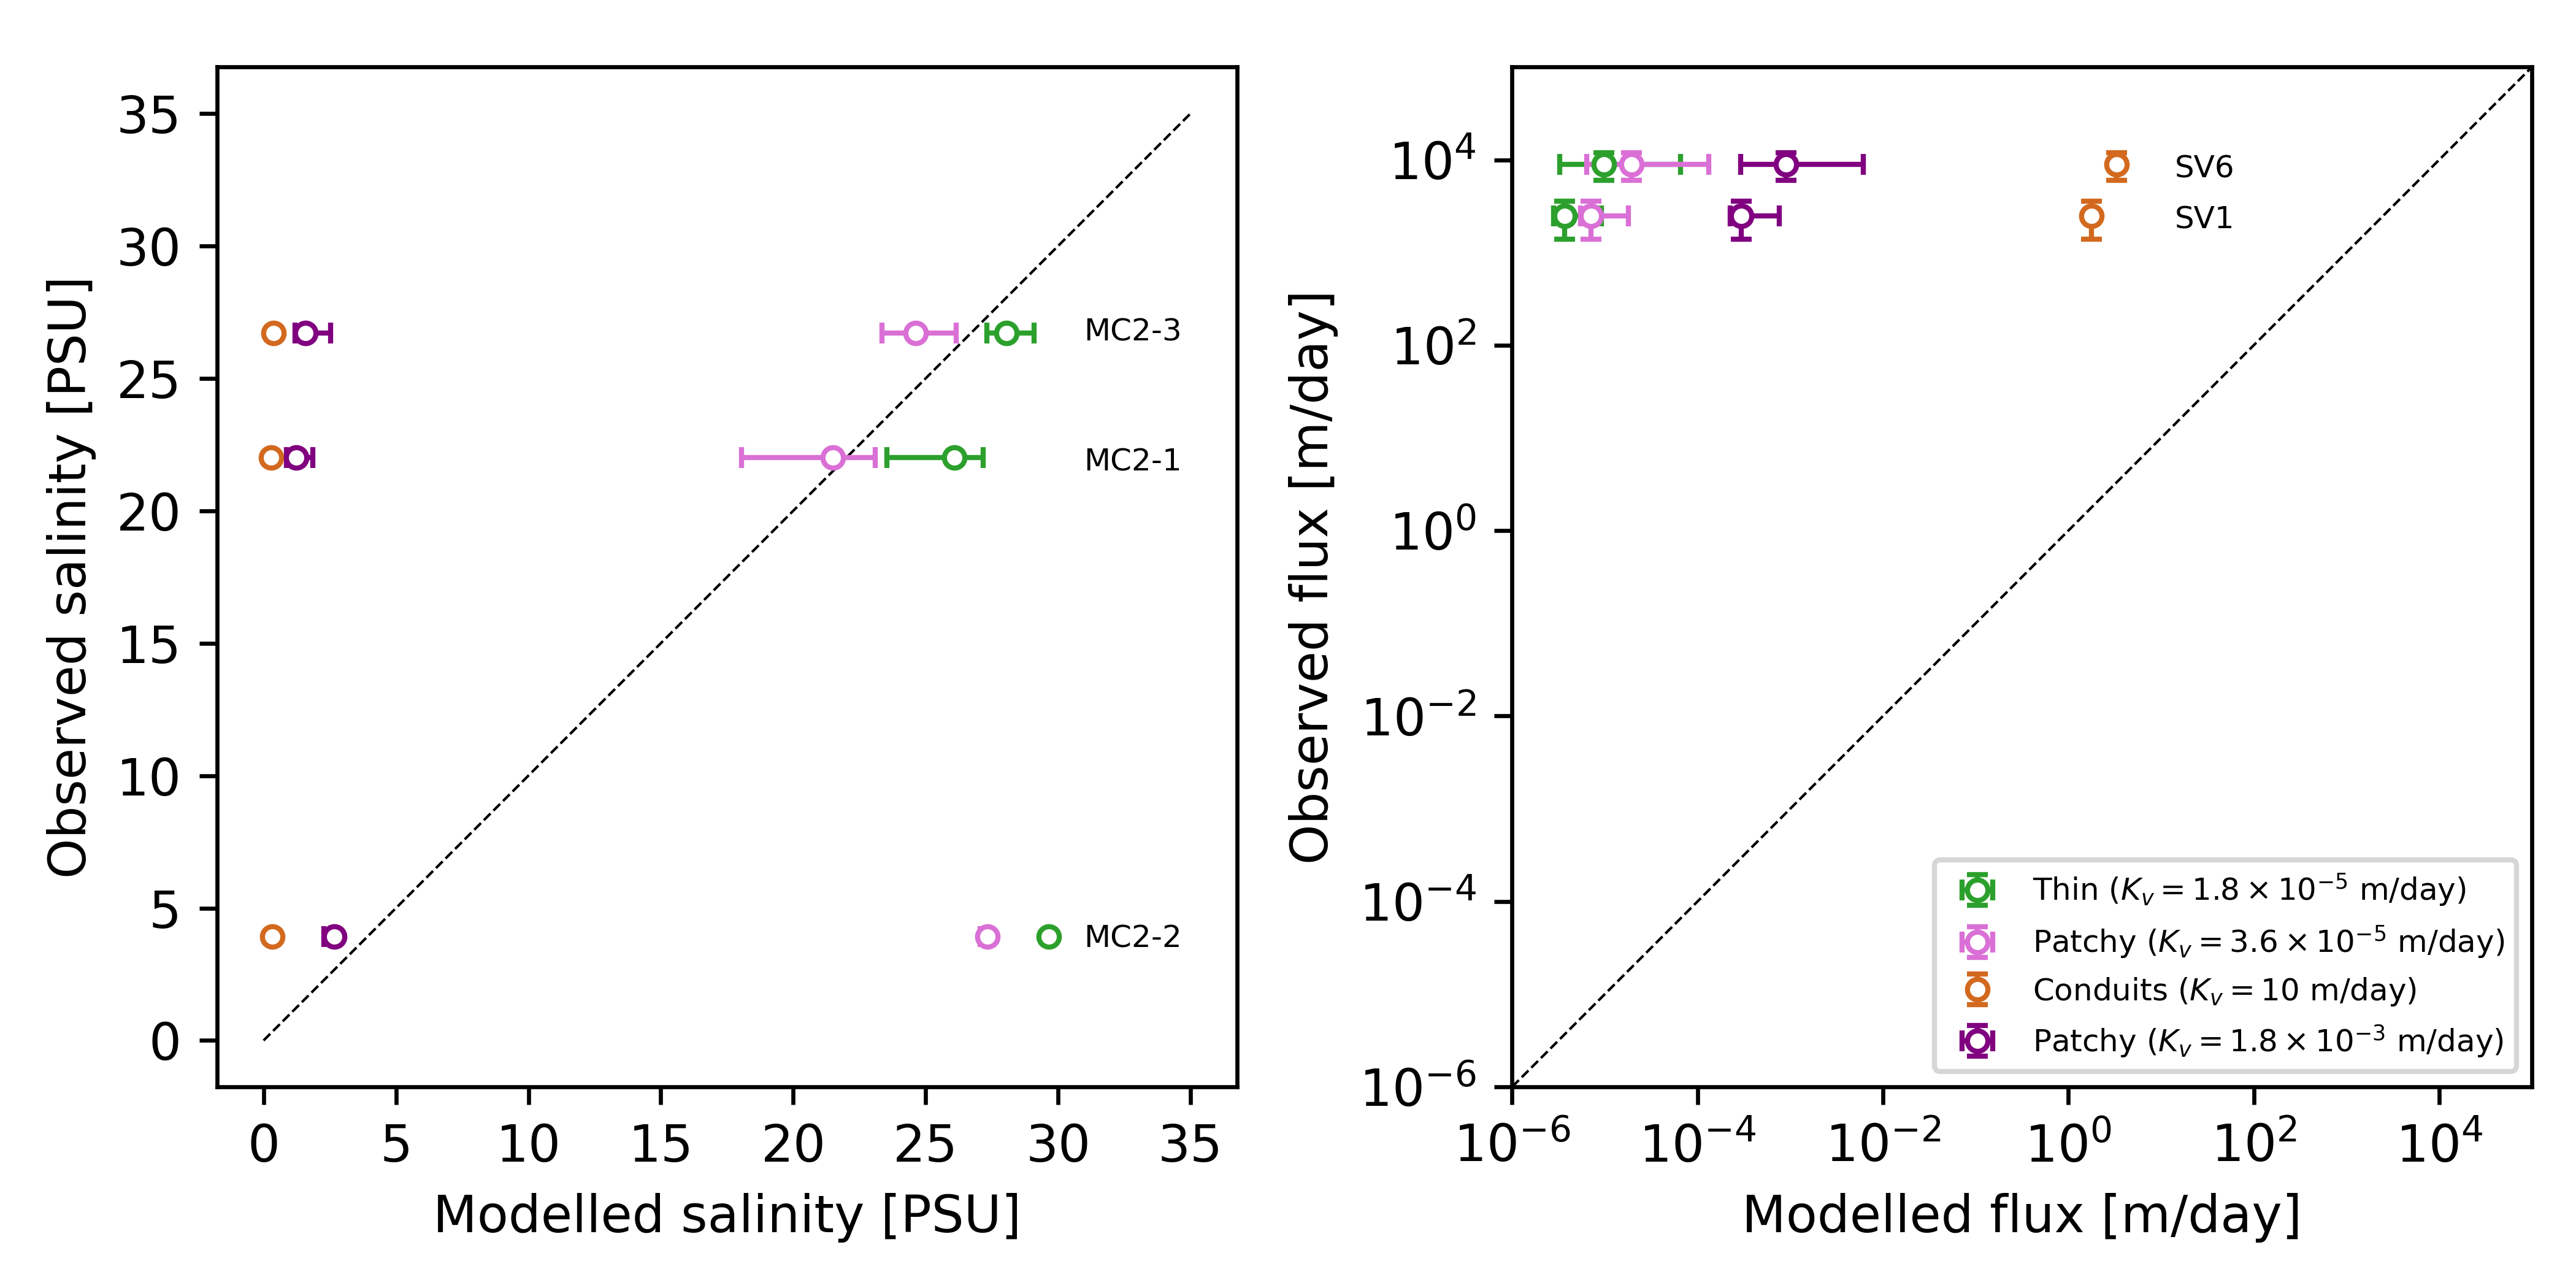
\includegraphics[width=0.9\textwidth]{multi_model_comparison_2.png}}
\caption{Comparison between modeled and observed fluxes and salinities, including an extra Patchy Aquitard model where the hydraulic conductivity of the patches is increased by a factor of 100.}
\label{fig:pockmarks_extra_comparison}
\end{figure}

\\

\noindent For this additional Patchy aquitard model, and the models presented in the main text, an additional Aquifer Depletion scenario was run.
This scenario has the same conditions as the original Aquifer Depletion scenario (Main text, Table 1), but was run for a longer period of 10 years.
In this scenario, more salinization occurred in the Aquitard Conduits model, and a small amount of salinization occurred in the Patchy Aquitard model with the higher hydraulic conductivity increase ($K_v = 1.8 \times 10^{-3}$ m/day).
\\

\noindent For the Patchy Aquitard model with only a small increase in hydraulic conductivity ($K_v = 3.6 \times 10^{-5}$ m/day), the 5 \% salinity contour is higher in the aquitard when compared to the Thin Aquitard model, suggesting that less seawater intrusion is occurring.
This reflects the fact that at steady-state, there is more upward flux in the Patchy Aquitard model and therefore less diffusion down into the aquifer compared with the Thin Aquitard model (Main text, Figure 7b,d).
While the flux downward through the pockmarks is greater for the Patchy Aquitard model, the steady-state conditions mean that even after 10 years of seawater intrusion, the aquitard is still fresher compared with the lower hydraulic conductivity Thin Aquitard model (Supporting Figure 5).

\begin{figure}[h!]
\centering
\makebox[\textwidth][c]{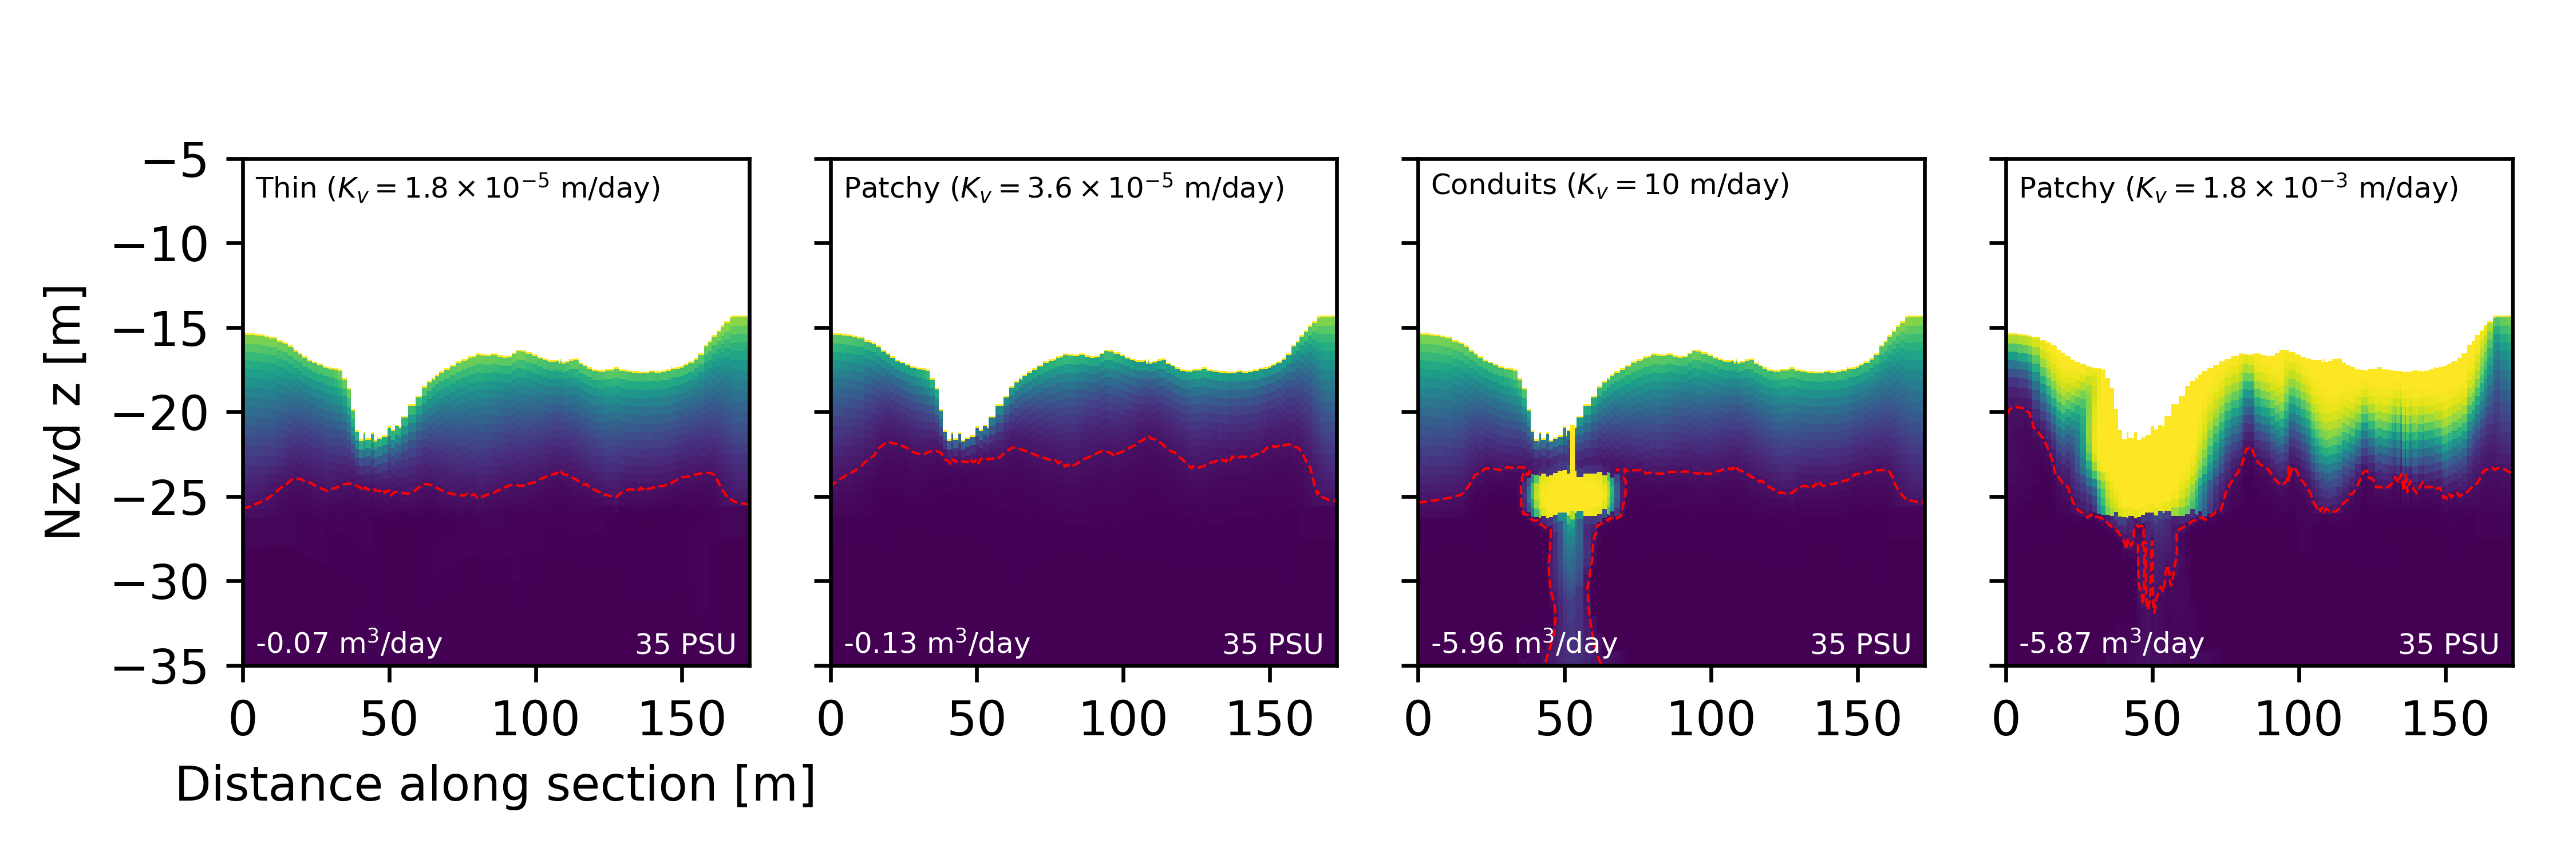
\includegraphics[width=1\textwidth]{longer_swi.png}}
\caption{Salinity distributions at Pockmark 6 after 10 years of aquifer depletion, for each geological model, including the extra Patchy Aquitard model with a greater hydraulic conductivity within the patches. The red dashed line shows 5 \% salinity contour.}
\label{fig:pockmarks_extra_long_swi}
\end{figure}

\pagebreak
\printbibliography


\end{document}
